\documentclass[english]{article}

\usepackage{graphicx}
\usepackage{alltt}
\usepackage{url}
\usepackage{tabularx}
%\usepackage{ngerman}
\usepackage{longtable}
\usepackage{color}
\usepackage{pdfpages}

\usepackage{xifthen}
\newboolean{showbackdoors}
\setboolean{showbackdoors}{true}  % set to false to hide subsection on backdoors for reviewing group


\newenvironment{prettytablex}[1]{\vspace{0.3cm}\noindent\tabularx{\linewidth}{@{\hspace{\parindent}}#1@{}}}{\endtabularx\vspace{0.3cm}}
%\newenvironment{prettytable}{\prettytablex{l X}}{\endprettytablex}



\title{\huge\sffamily\bfseries System Description and Risk Analysis}
\author{Cyrill Kr\"ahenb\"uhl \and Silvan Egli \and Lukas Bischofberger }
\date{}


\begin{document}
\maketitle

%% **** please observe the page limit **** 
%% (it is not allowed to change the font size or page geometry to gain more space)
%% comment or remove lines below before hand-in
\begin{center}
%{\large\textcolor{red}{Page limit: 30 pages.}}
\end{center}
%%%%%%%%%%%%%%%%%%%%%%%%%%%%%%%%%%%%%%%%%%%%%%

\tableofcontents
\pagebreak


\section{System Characterization}

\subsection{System Architecture}

Our system is a certificate authority. A user can retrieve his certificates, create new certificates and revoke certificates.

\begin{figure}[ht]
	\centering
	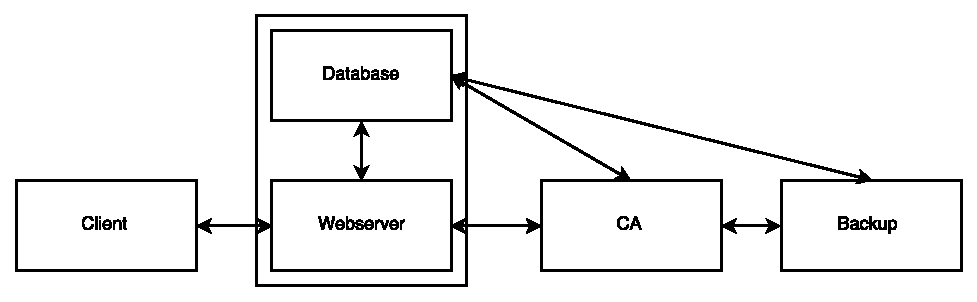
\includegraphics[scale=0.7]{seclabsystemoverview.pdf}
	\caption{System overview}
	\label{figure:systemoverview}
\end{figure}

The architecture is shown in figure \ref{figure:systemoverview}. All components except the client are in the same local network and are separated from the client by a firewall [siegli: are we using a dedicated machine (like a reverse proxy) or do we use a local firewalls on each machine ? in case of seperate machine I would put it into figure 1]. A client can only communicate with the system by connecting to the webserver. The webserver authenticates the user, manages the database and retrieves, creates or revokes certificates through the certificate authority (CA). The CA handles all certificate related operation. The backup server periodically backs up all data on the database and the CA.

%Describe the system's mission,  the system boundaries,
%and the overall system architecture, including the main subsystems and
%their relationships.   This description should provide a high-level
%overview of the system, e.g., suitable for managers, that complements
%the more technical description that follows.



%\subsection{System Functionality}

%Describe the system's functions.


%\subsection{Security Design}

%Describe the system's security design, including key and session management and security of data at rest and in transit.


\subsection{Components}

We divide our system into four major components.
\begin{itemize}
\item Client: The client side of the system is implemented using the Angular framework\footnote{https://angular.io/}.
\item Webserver \& Database: The webserver and the database run on the same Ubuntu system. For the webserver we use nginx\footnote{https://www.nginx.com/} and for the database mysql. The web application is implemented using the python framework Django\footnote{https://www.djangoproject.com/}.
\item CA server: The CA server runs on a Ubuntu system. All certificate related operations are implemented using openssl \footnote{https://www.openssl.org/}. The CA stores all certificates and their corresponding keys.
\item Backup server: The backup server runs on a Ubuntu system and uses rsync to synchronize certificates, keys and revocation lists from the CA and user informations from the database.
\end{itemize}

%List all system components and their interfaces, subdivided, for example, into categories such as platforms, applications, data records, etc. For  each component, state its relevant properties.
  

\subsection{Information Flows}


\begin{itemize}
	\item Client authentication: The client sends his username and password (or certificate) by using the client application to the webserver. The webserver (nginx) passes this information to the backend application (django) which then checks the username and password with help of the mysql database. If the user sent a certificate, this is checked by nginx. It must be ensured, that the certificate is valid and has not been revoked. Django then creates a JWT and returns it to the client application.
	
	\item Client certificate creation: The client checks in his view if he has already generated a key pair. Assuming he has, he sends a new certificate name to the webserver. Django requests a certificate from the CA server based on information from the database. The user is given the possibility to update his user information if he wants to. The CA server then creates the certificate based on the already present key pair and stores them safely. It returns the locations of these assets to django, which stores it in the database. Also it returns the message of the successful creation of the certificate to the client and offers the possibility to download the certificate, including the private key, in PKCS \#12 format.
	
	\item Certificate revocation: The client sends a revocation request to the webserver. Django asks the CA server to revoke the certificate, which then adds it to the revocation list. The CA server responds with  this updated revocation list.
\end{itemize}

\ifthenelse{\boolean{showbackdoors}}{
% show for handed-in version

%\subsection{Backdoors}
%
%Describe the implemented backdoors. 
%
%\bigskip\noindent
%\textbf{Hide this subsection in the version handed over to the reviewing team by setting the flag \texttt{showbackdoors} at the top of this document to \texttt{false}.}


%% do not delete the three lines below
}{ 
% empty for reviewing group's version
} 

%\subsection{Additional Material}
%
%You may have additional sections according to your needs.


\section{Risk Analysis and Security Measures}

\subsection{Assets}

%Describe the relevant assets and their required security properties. For example, data objects, access restrictions, configurations, etc.

Our project does not have physical assets. [siegli:  maybe we later have to make the assumption that the system is running on real machines. but for the moment i'm okay with that (let's see what they say ;-) ]  All the servers and networks are virtualized and thus will be listed as virtual assets. We will distinguish between software assets and information assets.

Software includes our virtual servers, including the software running on them. Further we count the connectivity of the different components as a logical asset as the network is also virtualized.

\begin{itemize}
	\item Frontend server: The frontend server runs a webserver and a database server. These are running an nginx and a mysql service on Ubuntu. Further our application is a django (python framework)  system which delivers the frontend (Angular) application. The packages and frameworks used are automatically updated with the newest security patches. The django application is updated by the system administrators.
	\item CA server: The backend server system consists of a bunch of bash scripts as well as the openssl package, both running on Ubuntu. The packages are automatically updated with the newest security patches.
	\item Backup server: The backup server runs rsync on Ubuntu, it is also automatically updated with the latest security patches.
	\item Availability of service / connectivity of the components: We rely on the virtualized network which is configured externally to work consistently [siegli: why consistently ?, lukasbi: if the network doesnt work consistently our app would have downtime] for our application to function. 
\end{itemize}

Our information assets include the following:

\begin{itemize}
	\item Certificates: This includes our own server and CA certificates as well as all the user generated certificates. Whereas the secrecy of the certificates is not critical, the security of the private keys is crucial. 
	\item User data: User data includes the users names, emails but also passwords. The security of this information is also critical to our application.
\end{itemize}

Further assets are the people working with the product. This includes the engineers building the platform and preserving the technical knowledge but also spans to the customers (employees of iMovie) using the product, wherein also originates the customer relation.   

\subsection{Risks and Vulnerabilities}

\begin{itemize}
    \item Weak passwords: 
    \begin{itemize}
        \item Users: Weak passwords of employees let advisories issue and revoking certificates in their names.
        \item System Administrator: Weak passwords of system administrators allow advisories access to the system with unbound possibilities.
    \end{itemize}
    \item Security Awareness and Knowledge of Employees: If the employees do not know how to request certificates and how to use them to sign/encrypt messages. This also includes the the protection of the private keys.
    \item Unavailability of CA: Threat actions like DOS attacks can make the CA unavailable. This results in making signing/verification of messages impossible as the public key of the CA can not be fetched. 
    \item Misconfiguration: The system administrator might expose the system to the outside by opening unintended ports for example.
    \item Threat sources: The iMovie company has a focus on investigative reporting. Depending on the subject being reported the threat source might include organized crime or governmental agency. 
    \item Information leakage: if confidential data (e.g. about a movie) is leaked customers might loose confidence.
    %\script 
\end{itemize}




%\paragraph{threats}

%\begin{itemize}
 %   \item key leakage
  %  \item user data leakage
   % \item compromise of webserver, ca server. backup server
    %\item unavailability
    %\item misbehaviour of trusted entities
%    \item sysadmin access to system
%\end{itemize}
    

%\paragraph{vulnerabilities}

%\begin{itemize}
 % \item misconfiguration of used software
 % \item bad passwords
 % \item badly implemented software (eg. access control)
 % \item zero days in used software
 % \item lack of security awareness of employees
 % \item sys admin access privileges
%\end{itemize}





%Name and describe potential threat sources including their motivation.

%\subsection{Risks Definitions}

%Define likelihood, impact and risk level using the following three tables.

%\subsubsection{Tools}

%\begin{center}
%\begin{tabular}{|l|l|}
%\hline
%\multicolumn{2}{|c|}{\bf Likelihood} \\
%\hline
%Likelihood & Description \\
%\hline
%\hline
%High   & \hspace*{20pt}\ldots \\
%\hline
%Medium & \hspace*{20pt}\ldots \\
%\hline
%Low   & \hspace*{20pt}\ldots \\
%\hline
%\end{tabular}
%\hspace{3em}
%\begin{tabular}{|l|l|}
%\hline
%\multicolumn{2}{|c|}{\bf Impact} \\
%\hline
%Impact & Description \\
%\hline
%\hline
%High   & \hspace*{20pt}\ldots \\
%\hline
%Medium & \hspace*{20pt}\ldots \\
%\hline
%Low   & \hspace*{20pt}\ldots \\
%\hline
%\end{tabular}
%\end{center}

%\vspace{5mm}

%\begin{center}
%\begin{tabular}{|l|c|c|c|}
%\hline
%\multicolumn{4}{|c|}{{\bf Risk Level}} \\
%\hline
%{{\bf Likelihood}} & \multicolumn{3}{c|}{{\bf Impact}} \\ %\cline{2-4}
%     & Low & Medium & High \\  \hline
% High & Low & Medium & High  \\
%\hline
% Medium & Low & Medium & Medium \\
%\hline
% Low & Low & Low & Low \\
%\hline
%\end{tabular}
%\end{center}


%\subsection{Risk Evaluation}
%
%List all potential threats and the corresponding countermeasures. Estimate the risk based on the information about the threat, the threat sources and the corresponding countermeasure. Adhere to the risk definitions you have given above.
%
%
%\subsubsection{{\it Evaluation Asset X}}
%
%Evaluate the likelihood, impact and the resulting risk,  \emph{after implementation of the corresponding countermeasures}. For each threat, clearly name the threat source and the the threat action.
%
%\begin{footnotesize}
%\begin{prettytablex}{llp{5.5cm}lll}
%No. & Threat &  Countermeasure(s) & L & I & Risk \\
%\hline
%1 & ... & ... & {\it Low} & {\it Low} & {\it Low} \\
%\hline
%2 & ... & ...& {\it Medium} & {\it High} & {\it Medium} \\
%\hline
%\end{prettytablex}
%\end{footnotesize}
%
%
%
%\subsubsection{{\it Evaluation Asset y}}
%
%\begin{footnotesize}
%\begin{prettytablex}{llp{5.5cm}lll}
%No. & Threat & Countermeasure(s) & L & I & Risk \\
%\hline
%1 & ... & ... & {\it Low} & {\it Low} & {\it Low} \\
%\hline
%2 & ... & ...& {\it Medium} & {\it High} & {\it Medium} \\
%\hline
%\end{prettytablex}
%\end{footnotesize}
%
%\subsubsection{Detailed Description of Selected Countermeasures}
%
%Optionally explain the details of the countermeasures mentioned above.
%
%
%
%\subsubsection{Risk Acceptance}
%
%List all medium and high risks, according to the evaluation above. For each risk, propose additional countermeasures that could be implemented to further reduce the risks.
%
%\begin{footnotesize}
%\begin{prettytablex}{p{2cm}X}
%No. of threat & Proposed additional countermeasure including expected impact  \\
%\hline
%... & ... \\
%\hline
%... & ... \\
%\hline
%\end{prettytablex}
%\end{footnotesize}

\end{document}

%%% Local Variables: 
%%% mode: latex
%%% TeX-master: "../../book"
%%% End: 
